%%%%%%%%%%%%%%%%%%%%%%%%%%%%%%%%%%%%%%%%%%%%%%%%%%%%%%%%%%%%%%%%%%%%%%%%%%%%%%
%%%%%%%%%%%%%%%%%%%%%%%%%%%%%%%%%%%%%%%%%%%%%%%%%%%%%%%%%%%%%%%%%%%%%%%%%%%%%%
%%
%% Ukázkový příklad dokumentace úkolu do předmětů IZP a IUS, 2010
%%
%% Upravená původní dokumentace od Davida Martinka.
%%%%%%%%%%%%%%%%%%%%%%%%%%%%%%%%%%%%%%%%%%%%%%%%%%%%%%%%%%%%%%%%%%%%%%%%%%%%%%
%%%%%%%%%%%%%%%%%%%%%%%%%%%%%%%%%%%%%%%%%%%%%%%%%%%%%%%%%%%%%%%%%%%%%%%%%%%%%%
\documentclass[12pt,a4paper,titlepage,final]{article}

% cestina a fonty
\usepackage[czech]{babel}
\usepackage[utf8]{inputenc}
% balicky pro odkazy
\usepackage[bookmarksopen,colorlinks,plainpages=false,urlcolor=blue,unicode]{hyperref}
\usepackage{listings}
\usepackage{url}
% obrazky
\usepackage[dvipdf]{graphicx}
% velikost stranky
\usepackage[top=3.5cm, left=2.5cm, text={17cm, 24cm}, ignorefoot]{geometry}

\begin{document}

%%%%%%%%%%%%%%%%%%%%%%%%%%%%%%%%%%%%%%%%%%%%%%%%%%%%%%%%%%%%%%%%%%%%%%%%%%%%%%
% titulní strana

% !!!!!!!!!!!!!!!!!!!!!!!!!!!!!!!!!!!!!!!!!!!!!!!!!
% změň následující údaje za své
\def\author{David Koňař}
\def\email{xkonar07@stud.fit.vutbr.cz}
\def\projname{Jednoduchý autentizační server}
% !!!!!!!!!!!!!!!!!!!!!!!!!!!!!!!!!!!!!!!!!!!!!!!!!

\begin{titlepage}

% \vspace*{1cm}
\begin{figure}[!h]
  \centering
  %
\includegraphics[height=5cm]{img/logo.eps}
  
\includegraphics[height=5cm]{logo.png}
\end{figure}

\vfill

\begin{center}
\begin{Large}
Dokumentace k projektu pro předmětu ISA\\
\end{Large}
\bigskip
\begin{Huge}
\projname\\
\end{Huge}
\end{center}

\vfill

\begin{center}
\begin{Large}
\today
\end{Large}
\end{center}

\vfill

\begin{flushleft}
\begin{large}
\begin{tabular}{ll}
Autor: & \author, \url{\email} \\
 & Fakulta Informačních Technologíí­ \\
 & Vysoké Učení­ Technické v~Brně \\
\end{tabular}
\end{large}
\end{flushleft}
\end{titlepage}


%%%%%%%%%%%%%%%%%%%%%%%%%%%%%%%%%%%%%%%%%%%%%%%%%%%%%%%%%%%%%%%%%%%%%%%%%%%%%%
% obsah
\pagestyle{plain}
\pagenumbering{roman}
\setcounter{page}{1}
\tableofcontents

%%%%%%%%%%%%%%%%%%%%%%%%%%%%%%%%%%%%%%%%%%%%%%%%%%%%%%%%%%%%%%%%%%%%%%%%%%%%%%
% textova zprava
\newpage
\pagestyle{plain}
\pagenumbering{arabic}
\setcounter{page}{1}



%%%%%%%%%%%%%%%%%%%%%%%%%%%%%%%%%%%%%%%%%%%%%%%%%%%%%%%%%%%%%%%%%%%%%%%%%%%%%%
%%%%%%%%%%%%%%%%%%%%%%%%%%%%%%%%%%%%%%%%%%%%%%%%%%%%%%%%%%%%%%%%%%%%%%%%%%%%%%
\section{Úvod} \label{uvod}
%%%%%%%%%%%%%%%%%%%%%%%%%%%%%%%%%%%%%%%%%%%%%%%%%%%%%%%%%%%%%%%%%%%%%%%%%%%%%%

Tato dokumentace popisuje návrch a implementaci jednoduchého RADIUS autentizačního serveru vytvořeného na základě projektu do předmětu ISA. Výsledný konzolový program přijímá jako parametr konfigurační soubor na jehož základě pak ověřuje autentizační požadavky na určitém rozhraní a portu. Klientům odešle zpět paket s odpovědí o výsledku procesu jeho autentizace.

Dokument obsahuje text členěný do několika částí. V následující kapitole \ref{oRadius} se zabývá přiblížením samotného RADIUS protokolu a formě paketů, kde dále v kapitole \ref{obecne} pokračuje základním nahlédnutím na obecnou implementaci řešení. V kapitole \ref{mojereseni} je pak již v rámci jednotlivých podkapitol na jednotlivé problémy nahlíženo podrobněji a vysvětlován princip jejich řešení a chodu serveru.
\newpage




%%%%%%%%%%%%%%%%%%%%%%%%%%%%%%%%%%%%%%%%%%%%%%%%%%%%%%%%%%%%%%%%%%%%%%%%%%%%%%
%%%%%%%%%%%%%%%%%%%%%%%%%%%%%%%%%%%%%%%%%%%%%%%%%%%%%%%%%%%%%%%%%%%%%%%%%%%%%%
\section{O protokolu RADIUS} \label{oRadius}
%%%%%%%%%%%%%%%%%%%%%%%%%%%%%%%%%%%%%%%%%%%%%%%%%%%%%%%%%%%%%%%%%%%%%%%%%%%%%%
RADIUS (\textit{Remote Authentication Dial In User Service}) protokol (specifikován v \textit{RFC 2865} \cite{rfc2865}) se obecně využívá pro vzdálenou autentizaci, autorizaci a účtování mezi serverem a klientem. Výhody tohoto protokolu spočívají v jeho bezpečnosti, neboť sdílené tajemství (\textit{shared secret}) se nikdy neposílá prostřednictví internetu a heslo pro přihlášení uživatele také není nikdy přenášeno ve formě čitelného textu, avšak spolu s dalšími parametry paketu je hashováno algoritmem MD5.

\subsection*{Formát RADIUS paketu}\label{paket_format}
Formát paketu RADIUS, popsán v kapitole 3, RFC 2865 určuje minimální velikost paketu na 20 bytů, kde pozice jednotlivých hodnot je právě v těchto prvních 20 bytech striktně určena jak zobrazuje obrázek níže.   
\begin{figure}[!h]
  \centering
  %
\includegraphics[height=5cm]{img/logo.eps}
  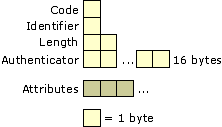
\includegraphics{RADIUS_packet.png}
  \caption{Názorné schéma formátu RADIUS paketu. Zdroj: \cite{paket}.}
\end{figure}



%%%%%%%%%%%%%%%%%%%%%%%%%%%%%%%%%%%%%%%%%%%%%%%%%%%%%%%%%%%%%%%%%%%%%%%%%%%%%%
%%%%%%%%%%%%%%%%%%%%%%%%%%%%%%%%%%%%%%%%%%%%%%%%%%%%%%%%%%%%%%%%%%%%%%%%%%%%%%
\section{Obecný pohled na implementaci}  \label{obecne}
%%%%%%%%%%%%%%%%%%%%%%%%%%%%%%%%%%%%%%%%%%%%%%%%%%%%%%%%%%%%%%%%%%%%%%%%%%%%%%
Program byl vyvíjen na operačním systému Ubuntu 12.04 LTS 32-bit, kde byl také testován. Během chodu programu nedochází k žádným výstupům na standardní či chybový výstup. K výpisu chyby a ukončení běhu serveru dochází jedině v případě fatální chyby spojené například s nenavázáním spojení, špatným formátem konfiguračního souboru - tedy při událostech, které by zásadně omezily chod celého serveru. V takovém případě, se server ukončí a zobrazí uživateli chybový stav, který způsobil přerušení chodu programu namísto toho, aby zůstal běžet s částečnou a nejistou konfigurací.

Zdrojové kódy programu se nachází ve dvou souborech \texttt{radauth.cpp} a \texttt{radauth.h}. V hlavičkovém souboru se nachází definice struktur, maker, inkluzi knihoven pro řádný chod programu. V prvním zmiňovaném souboru se pak nachází samotný algoritmus implementace RADIUS serveru.

Server běží v nepřetržité smyčce, dokud není násilně vypnut uživatelem (či systémem).



První byte určuje typ paketu - zda-li se jedná o např. \texttt{Access-request}, \texttt{Access-accept} či jiné. 2. byte obsahuje specifický identifikátor, pomocí nehož dochází ke spárování odeslaných požadavků a přijatých odpovědí v komunikaci.  3. - 4. byte obsahuje délku paketu. 5. - 20. byte je tzv. \textit{authenticator}, jenž obsahuje zahashovanou poslopnoustí řetězců (viz \cite{rfc2865}). Další prvky jsou atributy paketu které jsou volitelné a mohou či nemusí následovat. Různé atributy mohou být povinné v závislosti na typu paketu. 

\subsection{Příklad spuštění}


Program přijímá jeden povinný přepínač \texttt{-c} (program také akceptuje přepínač \texttt{–h}, jenž zobrazí informace o autorovi a příklad jak program spustit), který následuje cesta ke konfiguračnímu souboru. Cesta může být určena relativně či absolutně, avšak při neplatné cestě (soubor není nalezen), ukončí program svou činnost s chybovým hlášením. Konfigurační soubor, který zásadně ovlivňuje chod celého serveru, musí mít obsah v odpovídající formě: \texttt{atribut=hodnota}.
\begin{lstlisting}
./radauth -h
./radauth -c <konfiguracni_soubor>
\end{lstlisting}



%%%%%%%%%%%%%%%%%%%%%%%%%%%%%%%%%%%%%%%%%%%%%%%%%%%%%%%%%%%%%%%%%%%%%%%%%%%%%%
%%%%%%%%%%%%%%%%%%%%%%%%%%%%%%%%%%%%%%%%%%%%%%%%%%%%%%%%%%%%%%%%%%%%%%%%%%%%%%
\section{Vlastní řešení} \label{mojereseni}
%%%%%%%%%%%%%%%%%%%%%%%%%%%%%%%%%%%%%%%%%%%%%%%%%%%%%%%%%%%%%%%%%%%%%%%%%%%%%%

\subsection{Inicializace programu a zpracování se souborů}
Tato kapitola popisuje prvotní proces RADIUS serveru, který musí proběhnout ihned po spuštění – čtení uživatelských vstupních dat a nastavování počátečních hodnot.

Jak již bylo zmíněno výše, soubor obsahující nastavení musí dodržet předem danou formu (\texttt{atribut=hodota}). Jednotlivé vlastnosti musí být umístněné na samostatných řádcích a musí být vždy všechny (\texttt{userdb}, \texttt{secret}, \texttt{port}, \texttt{iface}) explicitně uvedeny. Program neuvažuje žádné výchozí hodnoty a při absenci některé z hodnot bude ukončen.

Parsování konfiguračního souboru je uživatelsky přívětivé do té podoby, že server akceptuje nadbytečné volné řádky, „bílé znaky“ a nehledí u názvů atributů na velikost písmen (je tzv. \textit{case-insensitive}).

Všechny atributy si program uloží (a tudíž již až do dalšího spuštění není konfigurační soubor pro server podstatný) a zpracuje je. Výjimkou z tohoto pravidla je atribut userdb, který obsahuje cestu k souboru s uživatelskými jmény a hesly (opět musí dodržet konvenci jeden záznam na jeden řádek, zde však ve formátu \texttt{jméno:heslo}), který se nenačítá ani nekontroluje dopředu, avšak je kontrolován až při příchozím požadavku na autentizaci. Toto chování umožňuje změnu, přidání, smazání uživatelů a jejich hesel za běhu programu bez nutnosti jeho vypínání, což je v případě serveru důležitá vlastnost. Problémem, který by snad mohl při současné editaci souboru s hesly a žádosti o čtení i ze strany serveru nastat je nemožnost jeho čtení – takový stav by se však promítl pouze do odmítnutí daného požadavku na autentizaci, který by již při opakovaném pokusu měl  proběhnout bez problémů.

\subsection{Komunikace server–klient}
Jakmile předchozí fáze spuštění programu je dokončena bez problémů, může se server pokusit připojit na definovaných rozhraních a portech a čekat na požadavky od klienta. Tuto část má na starost funkce \texttt{connect()}, jež otevírá socket, zjišťuje množství rozhraní, které se na počítači nachází a poté hledá uživatelem požadované rozhraní k jeho připojení a nastavení do neblokujícího režimy (k tomu je využita funkce \texttt{fcntl()} a přidání příznaku \texttt{O\_NONBLOCK}).

Jakmile jsou pro všechny rozhraní nastaveny odpovídající sockety (bez výskyty problému), přechází server, lze říci ze stále počáteční nastavovací fáze, do místa, kde již bude plnit svou předurčenou činnost. Program tedy nyní poběží v nekonečné smyčce, kde čeká, dokud na alespoň jednom z rozhraní nepřijde příchozí komunikace. Server následně zkontroluje na kterých rozhraních je potřeba vyhodnotit příchozí data. Zpracování probíhá prostřednictvím funkcí \texttt{processIncome()}, kde dochází k vyhodnoce přijatých dat a jejich analýze. Výsledek této verifikace navrací zpět a je volána funkce \texttt{createResponse()}, která na základě předchozích výstupů vytvoří odpovídající odpověď pro klienta. Třetí možností, která může nastat je naprosto neplatný (pro náš server) formát paketu, který program jednoduše zahodí a čeká na další příchozí data.
			   
\subsection{Velikost, typ a další podstatné náležitosti paketu}
Server neobsahuje komplexní řešení pro práci s RADIUS pakety, avšak, dle zadání, se zaměřije pouze na některé z prvků, jež mohou tyto pakety pojmout. Velikost paketu (jak již i byla zmíněna v kapitole \ref{paket_format}) není v této implementaci nijak ovlivněna a musí splňovat podmínku minimální velikosti 20 bytů a maximální velikost 4096 bytů. Při nedodržení této podmínky, či nesouladu mezi údaji o velikosti paketu, dochází k zahození na straně serveru a klinetskému stroji nebude odeslána žádná odpověď.

Typ paketu, který je programem zpracován je pouze \texttt{Access-request}, který je uchován v 1. bytu paketu a je vyjádřen numerickou hodnotou \texttt{1}. Veškerá ostatní komunikace je serverem ignorována.

\newpage			   




%%%%%%%%%%%%%%%%%%%%%%%%%%%%%%%%%%%%%%%%%%%%%%%%%%%%%%%%%%%%%%%%%%%%%%%%%%%%%%
%%%%%%%%%%%%%%%%%%%%%%%%%%%%%%%%%%%%%%%%%%%%%%%%%%%%%%%%%%%%%%%%%%%%%%%%%%%%%%
% seznam citované literatury: každá položka je definována příkazem
% \bibitem{xyz}, kde xyz je identifikátor citace (v textu použij: \cite{xyz})
\begin{thebibliography}{99}

% jedna citace:
\bibitem{rfc2865}RFC2865 - Remote Authentication Dial In User Service (RADIUS). \emph{IETF Tools} [online]. [June 2000] [cit. 2012-11-17]. Dostupné z: http://tools.ietf.org/html/rfc2865

\bibitem{paket}RADIUS Packet Format. \emph{MICROSOFT}. Microsoft TechNet [online]. 2012 [cit. 2012-11-17]. Dostupné z: http://technet.microsoft.com/en-us/library/cc958030.aspx

%\bibitem{kalendar}
%BLACKBURN, B.~J.; HOLFORD-STREVENS, L.: \emph{The Oxford Companion to the
%  Year}. Oxford: Oxford University Press, 1999, ISBN 0-19-214231-3.


\end{thebibliography}
\newpage



%%%%%%%%%%%%%%%%%%%%%%%%%%%%%%%%%%%%%%%%%%%%%%%%%%%%%%%%%%%%%%%%%%%%%%%%%%%%%%
%%%%%%%%%%%%%%%%%%%%%%%%%%%%%%%%%%%%%%%%%%%%%%%%%%%%%%%%%%%%%%%%%%%%%%%%%%%%%%
% přílohy
\appendix

\section{Metriky kódu} \label{metriky}
\paragraph{Počet souborů:} 2 soubory
\paragraph{Počet řádků zdrojového textu:} 238 řádků
\paragraph{Velikost statických dat:} 3328B
\paragraph{Velikost spustitelného souboru:} 9434B (systém Linux, 32 bitová
architektura)

\end{document}
